\subsection{Harmonický oscilátor}
	\begin{enumerate}
		\item
			Použitím WKB metody nalezněte spektrum a odpovídající vlnové funkce jednorozměrného harmonického oscilátoru
			popsaného (již známým) Hamiltoniánem
			\begin{equation}
			\operator{H}
				=\frac{1}{2M}\operator{p}^{2}+\frac{1}{2}M\Omega^{2}\operator{x}^{2}
			\end{equation}
			($M$ je hmotnost částice, která se v potenciálu pohybuje, $\Omega$ úhlová frekvence kmitů).
		
		\item
			Nakreslete graf vlnové funkce pro dvacátou energetickou hladinu ($n=20$) a porovnejte s přesnou vlnovou funkcí, která je řešením Schrödingerovy rovnice a která je
			určena Hermitovými polynomy
			\begin{equation}
			\phi_{n}(x)
				=\sqrt[4]{\frac{M\Omega}{\pi\hbar}}\frac{1}{\sqrt{n!2^{n}}}\,
					H_{n}(\xi)\,\e^{-\xi^{2}},\quad\xi=\sqrt{\frac{M\Omega}{\hbar}}x.
			\end{equation}
		
		\item
			Na základě tohoto srovnání diskutujte přesnost WKB metody.
	\end{enumerate}

\begin{solution}
	\begin{figure}[!htbp]
	\centering
	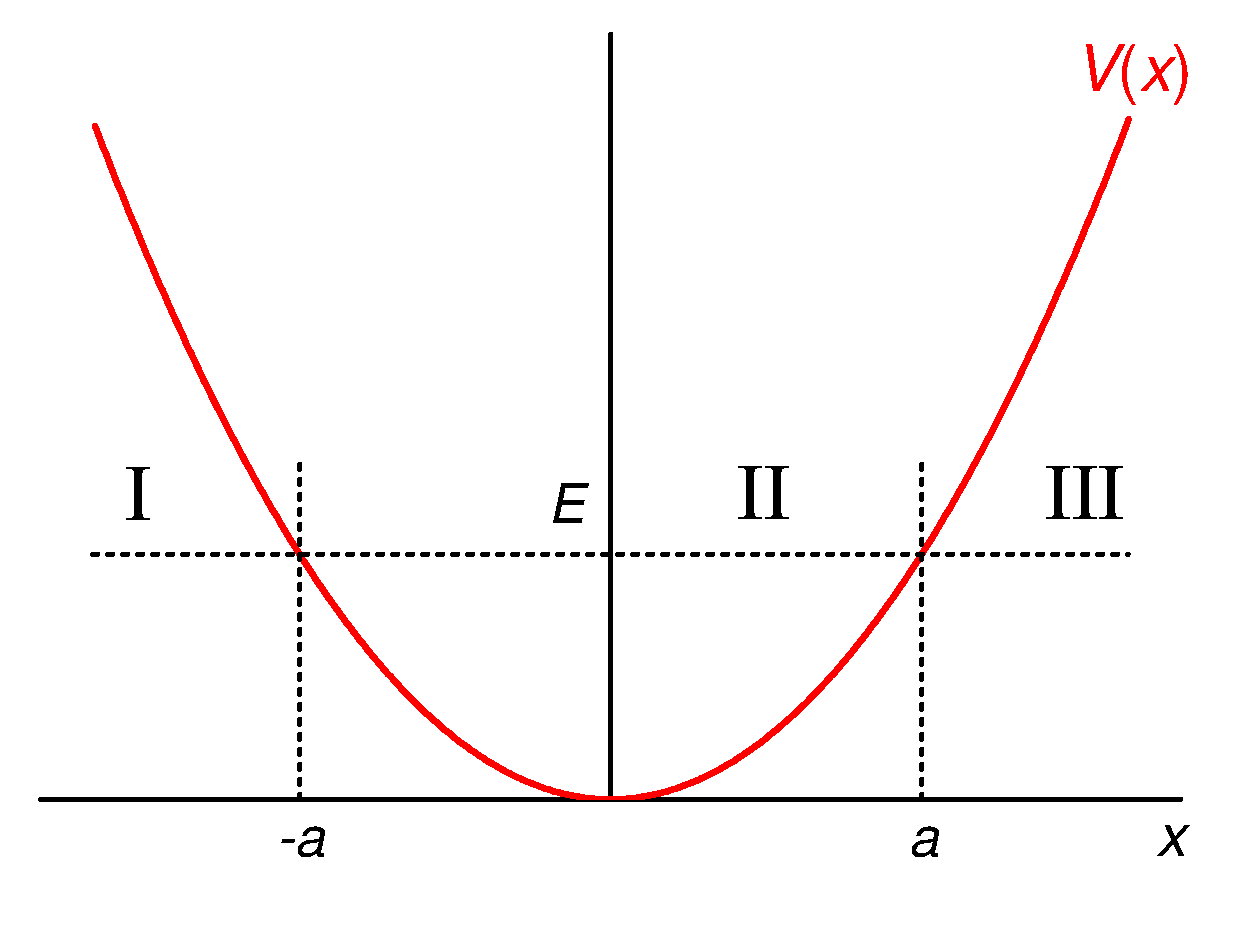
\epsfig{file=figures/ho.eps,width=0.6\linewidth,keepaspectratio}
	\caption{
		Potenciál harmonického oscilátoru s vyznačenými oblastmi pro WKB řešení.
	}
	\label{fig:WKBHarmonicOscillator}
	\end{figure}	
		
	Potenciál harmonického oscilátoru je znázorněn na obrázku~\ref{fig:WKBHarmonicOscillator}.
	Body obratu jsou $\pm a$, kde
	\begin{equation}
		a=\sqrt{\frac{2E}{M\Omega^{2}}}.
	\end{equation}
	Vlnová funkce v oblasti I (III) musí být WKB vlna, která ubývá pro $x\rightarrow-\infty$ ($x\rightarrow\infty$), takže
	\begin{subequations}
		\begin{align}
			\psi_{\mathrm{I}}(x)&=\frac{C}{\sqrt{\abs{p(x)}}}\e^{-\frac{1}{\hbar}\int_{x}^{-a}\abs{p(x')}\d x'}\equiv\lambda\e^{-I_{x}^{-a}},\\
			\psi_{\mathrm{III}}(x)&=\lambda'\e^{-I_{a}^{x}},
		\end{align}				
	\end{subequations}
	kde jsme použili značení~\eqref{eq:WKBNotation}.
	Klasická hybnost je
	\begin{equation}
		p(x)=\sqrt{2M\left(E-\frac{1}{2}M\Omega^{2}x^{2}\right)}.
	\end{equation}	
	Pomocí sešívacích vztahů~\eqref{eq:WKBConnectionDown1} se napojí vlnová funkce v oblasti II:
	\begin{equation}
		\psi_{\mathrm{II}}(x)=2\lambda\sin{\left[I_{-a}^{x}+\frac{\pi}{4}\right]}=2\lambda'\sin{\left[I_{x}^{a}+\frac{\pi}{4}\right]}.
	\end{equation}
	Vychází tedy $\lambda=-\lambda'$ a
	\begin{equation}
		\label{eq:WKBHarmonicOscillatorBS}
		I_{-a}^{a}=\pi\left(n+\frac{1}{2}\right),
	\end{equation}
	což je Bohrova-Sommerfeldova kvantovací podmínka.
	
	Zbývá spočítat integrál
	\begin{align}
		I_{x_{1}}^{x_{2}}
			&=\frac{1}{\hbar}\int_{x_{1}}^{x_{2}}p(x)\d x=\frac{1}{\hbar}\int_{x_{1}}^{x_{2}}\sqrt{2M\left(E-\frac{1}{2}M\Omega^{2}x^{2}\right)}\nonumber\\
			&=\frac{\sqrt{2ME}}{\hbar}\int_{x_{1}}^{x_{2}}\sqrt{1-\underbrace{\frac{M\Omega^{2}}{2E}}_{\frac{1}{a^{2}}}x^{2}}\,\d x=\equationcomment{y=\frac{x}{a} \\ \d x=a\d y}\nonumber\\
			&=\frac{2E}{\hbar\Omega}\int_{\frac{x_{1}}{a}}^{\frac{x_{2}}{a}}\sqrt{1-y^{2}}\,\d y,
	\end{align}
	přičemž primitivní funkce k poslednímu integrálu je
	\begin{align}
		\int\sqrt{1-y^{2}}\,\d y
			&=\equationcomment{y=\sin{z} \\ \d y=\cos{z} \d z}=\int\sqrt{1-\sin^{2}z}\,\cos{z}\,\d z\nonumber\\
			&=\int\cos^{2}\,\d z=\int\frac{1+\cos{2z}}{2}\d z=\frac{1}{2}\left(z+\frac{1}{2}\sin{2z}\right)\nonumber\\
			&=\frac{1}{2}\left(z+\sin{z}\cos{z}\right)=\frac{1}{2}\left(\arcsin{y}+y\sqrt{1-y^{2}}\right),
			\label{eq:intsqrt}
	\end{align}
	takže
	\begin{equation}
		I_{x_{1}}^{x_{2}}=\frac{E}{\hbar\Omega}\left[\arcsin{y}+y\sqrt{1-y^{2}}\right]_{\frac{x_{1}}{a}}^{\frac{x_{2}}{a}}.
	\end{equation}
	Po dosazení vyjádření tohoto integrálu do kvantovacích podmínek~\eqref{eq:WKBHarmonicOscillatorBS} vychází
	\begin{align}
		I_{-a}^{a}&=\frac{E}{\hbar\Omega}\pi=\pi\left(n+\frac{1}{2}\right) && \Longrightarrow & E_{n}=\hbar\Omega\left(n+\frac{1}{2}\right),
	\end{align}
	což je přesné spektrum harmonického oscilátoru.

	Zbývá určit ještě vlnové funkce.
	V oblasti II je
	\begin{align}
		\psi_{\mathrm{II}}(x)
			&=2\lambda\sin{\left\{\frac{E}{\hbar\Omega}\left[\arcsin{y}+y\sqrt{1-y^{2}}\right]_{\frac{x}{a}}^{\frac{a}{a}=1}+\frac{\pi}{4}\right\}}\nonumber\\
			&=2\lambda\sin{\left[\frac{E}{\hbar\Omega}\left(\underbrace{\frac{\pi}{2}-\arcsin{\frac{x}{a}}}_{\arccos{\frac{x}{a}}}-\frac{x}{a}\sqrt{1-\frac{x^{2}}{a^{2}}}\right)+\frac{\pi}{4}\right]}\nonumber\\
			&=\frac{2C}{\sqrt{p(x)}}\sin\left[\frac{E}{\hbar\Omega}\left(\arccos{\frac{x}{a}}-\frac{x}{a}\sqrt{1-\frac{x^{2}}{a^{2}}}\right)+\frac{\pi}{4}\right].
	\end{align}
	
	V klasicky zakázaných oblastech I a III vychází integrál
	\begin{align}
		I_{x_{1}}^{x_{2}}
			&=\frac{2E}{\hbar\Omega}\int_{\frac{x_{1}}{a}}^{\frac{x_{2}}{a}}\sqrt{y^{2}-1}\,\d y
			 =\frac{E}{\hbar\Omega}\left[-\arccosh{y}+y\sqrt{y^{2}-1}\right]_{\frac{x_{1}}{a}}^{\frac{x_{2}}{a}}\nonumber\\
			&=\frac{E}{\hbar\Omega}\left[-\ln{\left(y+\sqrt{y^{2}-1}\right)}+y\sqrt{y^{2}-1}\right]_{\frac{x_{1}}{a}}^{\frac{x_{2}}{a}},
	\end{align}
	takže	
	\begin{align}
		\psi_{\mathrm{I}}(x)
			&=(-1)^{n}\lambda\exp\left\{-\frac{E}{\hbar\Omega}\left[-\underbrace{\ln{\left(y+\sqrt{y^{2}-1}\right)}}_{\ln(-z)=\ln{\abs{z}}+\im\pi}+y\sqrt{y^{2}-1}\right]_{\frac{x}{a}}^{-1}\right\}\nonumber\\
			&=(-1)^{n}\frac{C}{\sqrt{\abs{p(x)}}}\e^{\frac{E}{\hbar\Omega}\left[\ln{\left(-\frac{x}{a}+\sqrt{\frac{x^{2}}{a^{2}}-1}\right)}+\frac{x}{a}\sqrt{\frac{x^{2}}{a^{2}}-1}\right]}
	\end{align}
	a
	\begin{align}
		\psi_{\mathrm{III}}(x)
			&=\lambda\e^{-\frac{E}{\hbar\Omega}\left[-\arccosh{y}+x\sqrt{y^{2}-1}\right]_{1}^{\frac{x}{a}}}
			 =\frac{C}{\sqrt{\abs{p(x)}}}\e^{-\frac{E}{\hbar\Omega}\left[-\arccosh{\frac{x}{a}}+\frac{x}{a}\sqrt{\frac{x^{2}}{a^{2}}-1}\right]}.
	\end{align}
	Konstanta $C$ se určí z normalizace, přičemž pro $n$ velké a $\hbar=\Omega=M=1$ konverguje k hodnotě $C\rightarrow1/\sqrt{2\pi}$.
	
	\begin{figure}[!htbp]
		\centering
		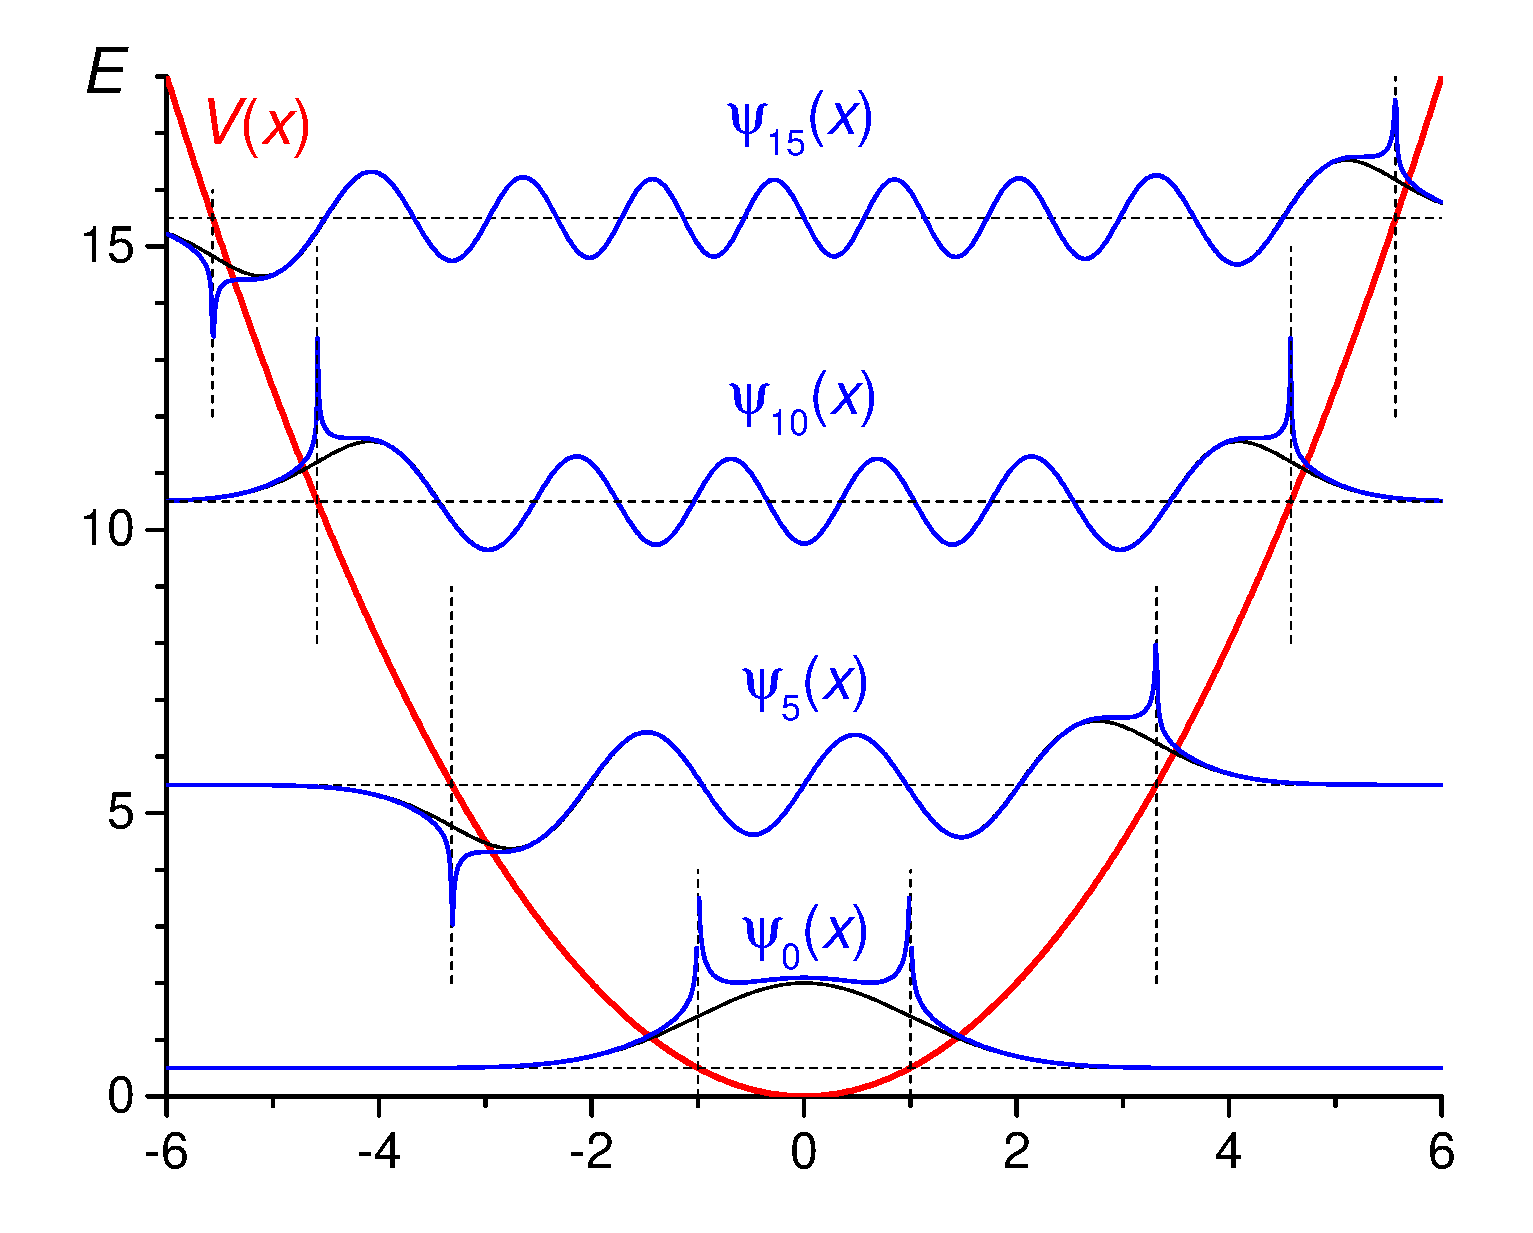
\epsfig{file=figures/howf.eps,width=0.7\linewidth,keepaspectratio}
		\scaption{
			Vlnové funkce harmonického oscilátoru s $\Omega=M=\hbar=1$ pro energie $E_{0}=\frac{1}{2}$, $E_{5}=\frac{11}{2}$, $E_{10}=\frac{21}{2}$, $E_{15}=\frac{31}{2}$.
			Přesné vlnové funkce dané Hermitovými polynomy jsou zobrazeny černými plnými čarami, odpovídající WKB aproximace jsou zobrazeny modrými plnými čarami
			(WKB vlnové funkce divergují v klasických bodech obratu, tj. v bodech, kde $E_{n}=V(x)$).
			WKB vlnové funkce jsou normalizované faktorem $1/\sqrt{2\pi}$.
		}
		\label{fig:howf}
	\end{figure}	
	
	Několik vlnových funkcí je znázorněno na obrázku~\ref{fig:howf}.
	Je vidět, že kromě bodu obratu WKB vlnová funkce velmi přesně aproximuje přesnou vlnovou funkci harmonickému oscilátoru.
\end{solution}